\setcounter{chapter}{1}
\chapter{フーリエ解析入門}
%
波動や振動現象など,何らかの系の状態を表す関数が周期的に振る舞うものは
私たちの身の周りに溢れている.
例えば,私たちに近い分野でみると,
種々の分光学的測定で得られる時系列データ(信号)は周期関数(とみなせるもの)である.
それらは一見するとグチャグチャしていて,ただ漠然と眺めているだけでは新しい知見は得られない.
そうではなく,例えば,その信号の中にはどういった振動数の波がどの程度含まれているか,
などを取り出すことが出来れば,その現象の理解を深めることができる.
その要求に答える数学的手法がフーリエ (Fourier)解析である.
この例に限らず,フーリエ解析は極めて広い分野で使われる強力な手法であり,
前章で学んだ微分方程式を解く際にも有効である.
そこで,この章ではフーリエ解析について学んでいくことにする.
ただし,「フーリエ解析」という名前で1期分の講義があるくらいで,
フーリエ解析に関する諸事項を幅広くかつ厳格に述べるには圧倒的に時間が足りないので,
かなり初歩的な事項を紹介するに留めざるを得ないが,それでも応用範囲は広い.

%しかし,
%ここでは,近い将来皆さんが化学工学の分野で研究を進めていてフーリエ解析
%の知識が必要に
%
\section{フーリエ級数}
%
皆さんにとって馴染みのあるテイラー展開について考えてみよう.
テイラー展開とは,次式のように
関数$f(x)$をべき級数として展開する,というものであった.
\begin{align}
  f\left(x\right) &= f\left(a\right) + f^{\prime}\left(a\right)
 \left(x-a\right) + \dfrac{f^{\prime\prime}\left(a\right)}{2!}\left(x-a\right)^{2} + \cdots. 
\end{align}
%
上述のように,テイラー展開ではべき級数となるが,$x^{0},~x^{1},~x^2,~x^3,\cdots$以外にも,何らかの関数のセットで展開出来るのではないか
と考えることは,一般性を重んじる(ことが多い)数学の立場からすると自然なことである.実際,そのような関数のセットを系統立てた考えの元に
用意することは可能で\footnote{このあたりの話はとても面白いのだが,時間の都合上省略する.興味が出た人は直交関数やグラム-シュミットの直交化法といったキーワードで調べてみると良い.決して難しくはない.},
関数のセットの一つとして,三角関数(sin, cos)が挙げられる.
周期関数を展開する際に,三角関数を用いるのはもっともらしいように思える.実は周期関数を三角関数を用いて展開して得られるものをフーリエ級数と呼び,これから学んでいくことになる.

まずは,周期関数について整理しておく.
周期$L~(>0)$の関数$f(x)$とは,
\begin{align}
  f\left(x + L\right) = f\left(x\right), 
\end{align}
を満たす関数のことを指す.
また,もし$a\leq x \leq b$の範囲で定義されている関数の場合は,
それを周期$b-a$の周期関数と一部とみなして,全区間に拡張することができる.
%
\begin{figure}[htbp]
  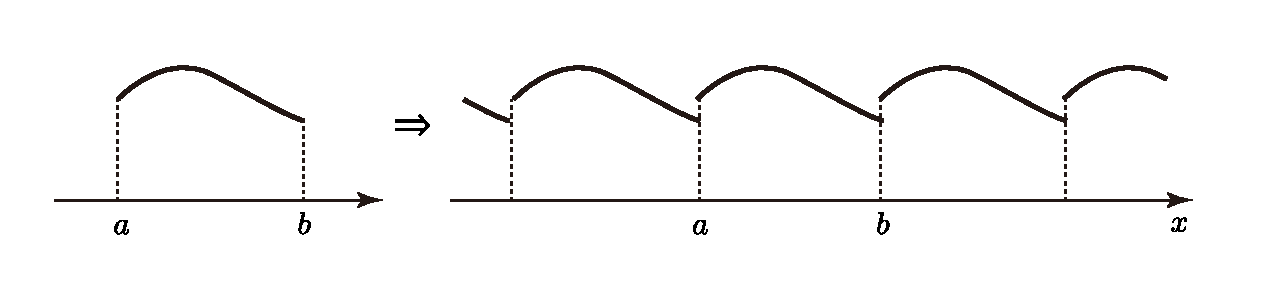
\includegraphics[width=1.0\linewidth]{figures/extend_function.eps} 
\end{figure}
%
\subsection{三角関数に関する諸公式}
%
フーリエ解析で現れる式変形では,割と高い頻度で高校数学で学んだタイプの三角関数の定理や積分
が現れる.それをその都度証明していくのは大変なので,ここで公式としてまとめておく.
\begin{align}
 &\sin\left(\alpha \pm \beta\right) = \sin\alpha \cos \beta \pm \cos\alpha \sin\beta, \\
 &\cos\left(\alpha \pm \beta\right) = \cos\alpha \cos \beta \mp \sin\alpha \sin\beta, \\
 &\sin^{2} \alpha = \dfrac{1-\cos 2\alpha}{2}, \\
 &\cos^{2} \alpha = \dfrac{1+\cos 2\alpha}{2}, \\
 &\sin \alpha \cos \beta = \dfrac{1}{2}\left(\sin(\alpha+\beta)+\sin\left(\alpha -\beta\right)\right), \label{tri_formula_01} \\
 &\sin \alpha \sin \beta = \dfrac{1}{2}\left(\cos(\alpha-\beta) - \cos(\alpha+\beta)\right). \label{tri_formula_02} 
\end{align}

また,$m,~n$を自然数として次式が成り立つ.
\begin{align}
 &\int_{0}^{2\pi}dx\,\cos nx = 0,  \label{tri_intformula_01} \\
 &\int_{0}^{2\pi}dx\,\sin nx = 0,  \label{tri_intformula_02} \\
 &\int_{0}^{2\pi}dx\,\cos mx \cos nx = 0\, \quad (m\neq n) \label{tri_intformula_03} \\
 &\int_{0}^{2\pi}dx\,\cos^{2} nx = \pi, \label{tri_intformula_04} \\
 &\int_{0}^{2\pi}dx\,\cos mx \sin nx = 0, \label{tri_intformula_05} \\
 &\int_{0}^{2\pi}dx\,\sin mx \sin nx = 0, \quad (m\neq n) \label{tri_intformula_06} \\
 &\int_{0}^{2\pi}dx\,\sin^{2} nx = \pi. \label{tri_intformula_07}
\end{align}
ここでは積分区間を$0\leq x \leq 2\pi$にしているが,これを定数分だけずらした区間$a\leq x \leq a + 2\pi$で
あっても上式は成り立つ.
%
\subsection{複素フーリエ級数}
%
それでは実際に周期関数をフーリエ級数の形で表すことを考えてみよう.
まず大事なことは,周期$L$の関数$f\left(x\right)$を展開するために用いる
三角関数も周期$L$の関数でなければならない,ということである.
$\sin x$, $\cos x$は周期$2\pi$の関数であるから,これらを周期$L$にするためには引数をいじって,
\begin{align}
  \sin\left(\dfrac{2\pi n}{L}x\right),\quad \cos\left(\dfrac{2\pi n}{L}x\right),
\end{align}
とすれば良い.ただし,$n$は整数である.ここでは,オイラーの公式を用いて,sin関数とcos関数をまとめて,
\begin{align}
 \exp\left(i\dfrac{2\pi n}{L}x\right),
\end{align}
にしておいて,$f\left(x\right)$を次式のように展開してみる.
\begin{align}
 f\left(x\right) = \sum_{n=-\infty}^{\infty} c_{n} \exp\left(i\dfrac{2\pi n}{L}x\right). 
\end{align}
これを複素フーリエ級数と呼ぶ.
級数展開では,その展開係数$c_m$を求めることが重要となるが,実は前節でまとめた公式を使うとすぐ求められる.
両辺に$\exp(-i\frac{2\pi m}{L}x)$をかけて,区間$-L/2 \leq x \leq L/2$で積分すると
\footnote{周期関数の場合は周期1つ分を含んでいれば良い.今回は対称性を意識して$-L/2 \leq x \leq L/2$としている.},左辺は
\begin{align}
\int_{-L/2}^{L/2}dx\,f\left(x\right)\exp\left(-i\dfrac{2\pi m}{L}x\right),
\end{align}
である(特に式変形はしていない).左辺は,
\begin{align}
 &\sum_{n=-\infty}^{\infty}c_n\int_{-L/2}^{L/2}dx\,\exp\left(-\dfrac{2\pi}{L}\left(n-m\right)x\right) \notag \\
 &=\sum_{n=\infty}^{\infty}c_n\int_{-L/2}^{L/2}dx\,\left\{\cos\left(\dfrac{2\pi}{L}\left(n-m\right)x\right) 
   + i\sin\left(\dfrac{2\pi}{L}\left(n-m\right)x\right)\right\},
\end{align}
である.ここで,$(2\pi/L)x = X$と変数変換すると,$dx = (L/2\pi)dX$であり,
積分区間は$-\pi\leq X \leq \pi$となるので,
\begin{align}
  \dfrac{L}{2\pi}  \sum_{n=-\infty}^{\infty} c_n \int_{-\pi}^{\pi}dX\, \left\{\cos\left(\left(n-m\right)X\right) + i\sin\left(\left(n-m\right)X\right)\right\},
\end{align}
である.$n=m$のときは,
\begin{align}
 \dfrac{L}{2\pi}  c_m \int_{-\pi}^{\pi}dX\, \left\{\cos\left(\left(n-m\right)X\right) + i\sin\left(\left(n-m\right)X\right)\right\} = \dfrac{L}{2\pi}c_{m}\int_{-\pi}^{\pi}dX = Lc_{m},
\end{align}
となり,$n\neq m$のときは\Eq{tri_intformula_01}と\Eq{tri_intformula_02}から,
\begin{align}
 \dfrac{L}{2\pi}   c_n \int_{-\pi}^{\pi}dX\, \left\{\cos\left(\left(n-m\right)X\right) + i\sin\left(\left(n-m\right)X\right)\right\} = 0, 
\end{align}
となる.結局生き残るのは$n=m$の項だけとなり,
\begin{align}
  c_m = \dfrac{1}{L}\int_{-L/2}^{L/2}dx\,f\left(x\right)\exp\left(-i\dfrac{2\pi m}{L}x \right), 
\end{align}
を得る.これが複素フーリエ級数の展開係数の表式である.この展開係数のことをフーリエ係数と呼ぶ.
今後の便宜のため,式を以下にまとめておく.
\begin{align}
 & f\left(x\right) = \sum_{n=-\infty}^{\infty} c_{n} \exp\left(i\dfrac{2\pi n}{L}x\right), \label{complex_fourier}\\
 & c_n = \dfrac{1}{L}\int_{-L/2}^{L/2}dx\,f\left(x\right)\exp\left(-i\dfrac{2\pi n}{L}x \right). \label{complex_fourier_coef}
\end{align}
%
\subsection{実フーリエ級数}
%
複素フーリエ級数は,$\exp(i\frac{2\pi n}{L}x)$を展開に用いているが,
これを$\sin(\frac{2\pi n}{L}x)$と$\cos(\frac{2\pi n}{L}x)$で表してみよう.
\Eq{complex_fourier}の和を$n=0$, $n=-\infty\sim -1$, $n=1\sim \infty$に分けてみると,
\begin{align}
  f\left(x\right)
  &= c_{0} + \sum_{n=-\infty}^{-1}c_n \exp\left(i\dfrac{2\pi n }{L}x\right) 
    + \sum_{n=1}^{\infty} c_n \exp\left(i\dfrac{2\pi n }{L}x\right) \notag \\
  &= c_{0} + \sum_{n=1}^{\infty}c_{-n}\exp\left(-i\dfrac{2\pi n}{L}x\right) 
   + \sum_{n=1}^{\infty}c_{n} \exp\left(i\dfrac{2\pi n}{L}x\right) \notag \\
  &= c_{0} + \sum_{n=1}^{\infty}\left\{\left(c_n + c_{-n}\right)\cos\left(\dfrac{2\pi n}{L}x\right)
           + i\left(c_n - c_{-n}\right) \sin\left(\dfrac{2\pi n}{L}x\right)\right\}
\end{align}
ここで,
\begin{align}
  & a_n = c_{n} + c_{-n}, \\
  & b_n = i\left(c_n - c_{-n}\right), 
\end{align}
を定義すると,
\begin{align}
  f\left(x\right) = \dfrac{a_0}{2} 
                  + \sum_{n=1}^{\infty}\left\{a_n \cos\left(\dfrac{2\pi n}{L}x\right)
                                             +b_n \sin\left(\dfrac{2\pi n}{L}x\right)\right\}, 
\end{align}
となる.上式を実フーリエ級数と呼ぶ.$a_n$と$b_n$の表式は,\Eq{complex_fourier_coef}から式変形することで出せる.
$a_n$については,
\begin{align}
  a_n &= \dfrac{1}{L}\int_{-L/2}^{L/2}dx\,f\left(x\right)
        \left\{\exp\left(i\dfrac{2\pi n}{L}x\right)
        +      \exp\left(-i\dfrac{2\pi n}{L}x\right)\right\} \notag \\
      &= \dfrac{2}{L}\int_{-L/2}^{L/2}dx\,f\left(x\right)\cos\left(\dfrac{2\pi n}{L}x\right), 
\end{align}
となる.$b_n$も同様にして求めることができて,
\begin{align}
  b_n = \dfrac{2}{L}\int_{-L/2}^{L/2}dx\,f\left(x\right)\sin\left(\dfrac{2\pi n}{L}x\right), 
\end{align}
である.
実フーリエ級数の式を以下にまとめておく.
\begin{align}
 & f\left(x\right) = \dfrac{a_0}{2} 
                   + \sum_{n=1}^{\infty}\left\{a_n \cos\left(\dfrac{2\pi n}{L}x\right)
                                             +b_n \sin\left(\dfrac{2\pi n}{L}x\right)\right\}, \\ 
 & a_n = \dfrac{2}{L}\int_{-L/2}^{L/2}dx\,f\left(x\right)\cos\left(\dfrac{2\pi n}{L}x\right), \\
 & b_n = \dfrac{2}{L}\int_{-L/2}^{L/2}dx\,f\left(x\right)\sin\left(\dfrac{2\pi n}{L}x\right).
\end{align}
式変形を追えば分かる通り,複素フーリエ級数と実フーリエ級数は等価である.
%
\subsection{フーリエ級数の展開可能性}
%
さて,ここまでは展開される$f(x)$の性質として周期性しか考えてこなかったが,
実際にはなんでも良いわけではなく,特定の条件を満たしている必要がある.もし,その条件を満たさない場合は,
級数が元々の関数$f(x)$に収束しなくなってしまう.
とはいえ,テイラー展開では,$f\left(x\right)$が何回でも微分可能であることが必要であったのに対し,
フーリエ級数では
係数が積分の形で表されているので,テイラー展開の場合よりも条件は厳しくない.
たとえ,不連続点や微分不可能な点があっても,そこで積分区間を分割して考えれば良いからだ.

フーリエ級数展開可能な周期関数$f(x)$は,その区間において「区分的になめらか」な関数であることが証明されている.
「区分的になめらか」とは,有限個の不連続点を除いて$f(x)$と$f^{\prime}(x)$が連続であり,
不連続点においても左側,右側極限が有限値をとることを指す.
例えば,下図左側の関数は不連続点が存在するが,区分的になめらかであるのに対し,
右側の関数は不連続点で発散しているので,区分的になめらかとは言えない.
\begin{figure}[htbp]
 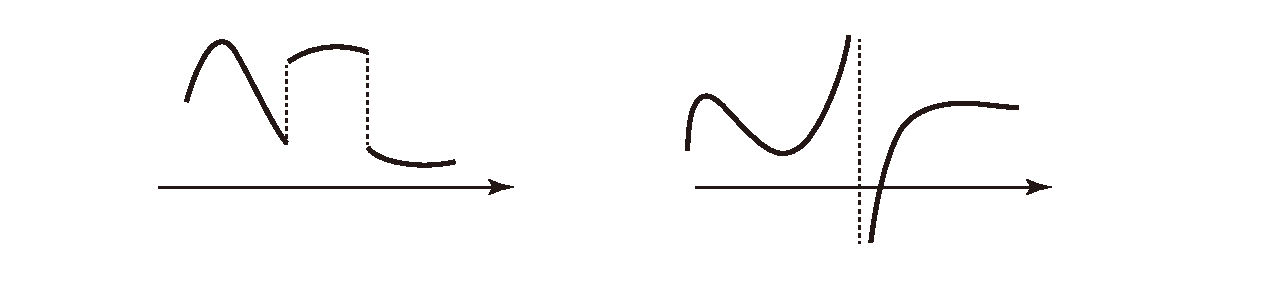
\includegraphics[width=1.0\linewidth]{figures/fourier_smooth.eps} 
\end{figure}
%
\newpage
%
\hrule
\reidai
次の関数$f(x)$をフーリエ級数展開せよ.
\begin{align}
  f\left(x\right) =
  \begin{cases}
    -1 & -1 \leq x < 0 \\
     1 & 0  \leq x < 1 
  \end{cases}. 
\end{align}
\vspace*{.2cm}
\hrule
\vspace*{.2cm}
複素フーリエ級数,実フーリエ級数どちらから出発しても良いが,
ここでは実フーリエ級数から式変形を進めることにする.
この関数の周期は$L=2$なので,
\begin{align}
 f\left(x\right) = \dfrac{a_0}{2} 
                   + \sum_{n=1}^{\infty}\left\{a_n \cos\left(n\pi x\right)
                                             +b_n \sin\left(n\pi x\right)\right\}.
\end{align}
まず,$a_n$は
\begin{align}
  a_n &= \int_{-1}^{1}dx\,f\left(x\right)\cos\left(n\pi x\right) 
       = -\int_{-1}^{0}dx\, \cos\left(n\pi x\right) + \int_{0}^{1}dx\,\cos\left(n\pi x\right) \notag \\
      &= 0,
\end{align}
である.次に,$b_n$は
\begin{align}
  b_n & = -\int_{-1}^{0}dx\,\sin\left(n\pi x\right) + \int_{0}^{1}dx\,\sin\left(n\pi x\right) \notag \\
      & = \dfrac{2}{\pi n}\left(1-\cos\left(\pi n\right)\right) \notag \\
      & = 
      \begin{cases}
	0 & n : 偶数 \\
        \dfrac{4}{\pi n} & n : 奇数
      \end{cases},
\end{align}
となる.
従って,
\begin{align}
 f\left(x\right) = \dfrac{4}{\pi}\sum_{n=1}^{\infty} \dfrac{1}{2n-1}\sin \left(\left(2n-1\right)\pi x \right),
\end{align}
が得られる.\\
\fbox{補足} 部分和で定義される関数
\begin{align}
 f_{M}(x) = \dfrac{4}{\pi}\sum_{n=1}^{M} \dfrac{1}{2n-1}
            \sin\left(\left(2n-1\right)\pi x\right),
\end{align}
を$M$を変えてプロットしてみると,次のようになる.
\begin{figure}[htbp]
 %\vspace*{-\intextsep}
 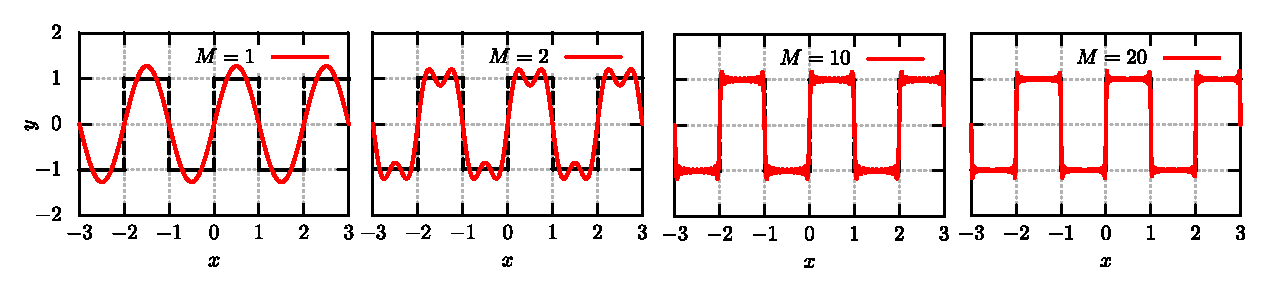
\includegraphics[width=1.0\linewidth]{figures/reidai01.eps} 
\end{figure}
%
\newpage
%
\subsection{フーリエ余弦級数,正弦級数}
%
時間$t$の$f(t)$を考える.
通常,時間の原点は測定開始時刻や何らかの化学現象が起きる(起こす)時刻にとることが多い.つまり,
$t>0$である.$f(t)$を全区間に拡張するとき,奇関数として拡張するか,
もしくは偶関数として拡張するかの2通りが考えられる.どちらを採用するのが良いかは注目している現象による.
区間$0\leq t \leq T$で定義された関数$f(t)$について,それぞれの場合で考えてみよう.\\
i) 偶関数に拡張した場合

フーリエ級数も偶関数になるはずである.
その場合は$\cos$関数だけで展開出来,フーリエ係数は,
\begin{align}
 a_n &= \dfrac{1}{L}\int_{-T}^{T}dt\,f\left(t\right)\cos\left(\dfrac{\pi n}{T}t\right) \notag \\
     &= \dfrac{2}{L}\int_{0}^{T}dt\, f\left(t\right)\cos\left(\dfrac{\pi n}{T}t\right), \\
 b_n & = 0, 
\end{align}
となる.偶関数に拡張したときのフーリエ級数をフーリエ余弦級数と呼ぶ.
\\
ii) 奇関数に拡張した場合

フーリエ級数も奇関数になるはずである.その場合は$\sin$関数だけで展開出来,
フーリエ係数は,
\begin{align}
  a_n & = 0, \notag \\
  b_n & = \dfrac{2}{L}\int_{0}^{T}dt\,f\left(t\right) \sin\left(\dfrac{\pi n}{T}t\right),
\end{align}
となる.奇関数に拡張したときのフーリエ級数をフーリエ正弦級数と呼ぶ.
%
%\newpage
%
%\hrule
%\reidai
%関数$f(x)=\sin x~(0\leq x \leq \pi)$のフーリエ余弦級数,フーリエ正弦関数級数を求めよ.
%つまり,$f(x)$を偶関数に拡張した場合と奇関数に拡張した場合のそれぞれでフーリエ級数を求めよ.
%\vspace*{.2cm}
%\hrule
%\vspace*{.2cm}
%
%まずは,余弦

\subsection{フーリエ積分}
%
これまでは周期関数を扱ってきたが,
その適用範囲を$-\infty\sim \infty$の区間で定義された
非周期関数$f(x)$に拡張することを考えてみる.
この取り組みが,後で学ぶフーリエ変換につながっていく.

$f(x)$として,
\begin{align}
 \int_{-\infty}^{\infty}dx\,\left|f\left(x\right)\right| = M < + \infty, 
\end{align}
つまり,この積分が有限値になることを要請する.

まずは,$f(x)$の定義区間を$-L/2\leq x \leq L/2$としておいて,
色々と式変形した後に$L\to \infty$に飛ばして,周期性をなくす,という戦略をとることにする.
このとき,$f(x)$の複素フーリエ級数は,
\begin{align}
  &f\left(x\right) = \sum_{n=-\infty}^{\infty}c_n \exp\left(i\dfrac{2\pi n}{L}x\right), \\
  &c_n = \dfrac{1}{L}\int_{-L}^{L}dx\,f\left(x\right)\exp\left(-i\dfrac{2\pi n}{L}x\right),
\end{align}
である.ここで,
\begin{align}
  \Delta u = \dfrac{2\pi}{L},
\end{align}
を定義すると,
\begin{align}
 f\left(x\right) &= \sum_{n=-\infty}^{\infty}c_n \exp\left(i\dfrac{2\pi n}{L}x\right) \notag \\
                 &= \sum_{n=-\infty}^{\infty}\left\{\dfrac{1}{L}\int_{-L/2}^{L/2}dt\, f\left(t\right)
                             \exp\left(-i\dfrac{2\pi n}{L}t\right)\right\}\exp\left(i\dfrac{2\pi n}{L}x\right) \notag \\
                 &= \sum_{n=-\infty}^{\infty}\left\{\dfrac{\Delta u}{2\pi}\int_{-L/2}^{L/2}dt 
                        f\left(t\right)\exp\left(-in\Delta u t\right)\right\}\exp\left(in\Delta u x\right),
\end{align}
と表せる.$L\to \infty$のとき,$\Delta u \to 0$であり,区分求積
\begin{align}
 \lim_{\Delta u\to 0} \sum_{n=-\infty}^{\infty}\Delta u F\left(n\Delta u\right) = \int_{-\infty}^{\infty}du\,F\left(u\right),
\end{align}
を用いると,
\begin{align}
 f\left(x\right) = \dfrac{1}{2\pi}\int_{-\infty}^{\infty}du\,
                   \left(\int_{-\infty}^{\infty}dt\,f\left(t\right)\exp\left(-iut\right)\right)\exp\left(iux\right), 
\end{align}
を得る.これをフーリエ積分と呼ぶ.
%
\newpage
%
\hrule
\reidai
以下の問いに答えよ.
\begin{enumerate}[(1)]
  \item 関数
	\begin{align}
	  f\left(x\right) =
	  \begin{cases}
	    1 & -1\leq x < 1 \\
	    0 & それ以外
	  \end{cases},
	\end{align}
	のフーリエ積分を求めよ.フーリエ積分は積分表示のままで良い.
  \item 次の積分を求めよ.
	\begin{align}
	  \int_0^{\infty}\dfrac{\sin x}{x}dx. 
	\end{align}
\end{enumerate}
\hrule

\begin{enumerate}[(1)]
  \item
	\begin{align}
	  \int_{-\infty}^{\infty}dt f(t)e^{-iut} = \dfrac{2\sin u}{u},
	\end{align}
      であるから,フーリエ積分は,
       \begin{align}
	 f(x) = \int_{-\infty}^{\infty}du\dfrac{\sin u}{\pi u}e^{iux}. 
       \end{align}
  \item (1)で求めたフーリエ積分に対し,$x=0$を代入すると,
	\begin{align}
	  & 1 = \int_{-\infty}^{\infty}du\, \dfrac{\sin u}{\pi u}, \notag \\
          &\rightarrow \int_{-\infty}^{\infty}du\, \dfrac{\sin u}{ u} = \pi.
	\end{align}
	$\sin u/u$は偶関数であるから,
	\begin{align}
	 \int_{0}^{\infty}du\, \dfrac{\sin u}{ u} = \dfrac{\pi}{2}, 
	\end{align}
	を得る.
\end{enumerate}
%
